% THIS IS SIGPROC-SP.TEX - VERSION 3.0
% WORKS WITH V3.1SP OF ACM_PROC_ARTICLE-SP.CLS
% JUNE 2007
%
% It is an example file showing how to use the 'acm_proc_article-sp.cls' V3.1SP
% LaTeX2e document class file for Conference Proceedings submissions.
% ----------------------------------------------------------------------------------------------------------------
% This .tex file (and associated .cls V3.1SP) *DOES NOT* produce:
%       1) The Permission Statement
%       2) The Conference (location) Info information
%       3) The Copyright Line with ACM data
%       4) Page numbering
% ---------------------------------------------------------------------------------------------------------------
% It is an example which *does* use the .bib file (from which the .bbl file
% is produced).
% REMEMBER HOWEVER: After having produced the .bbl file,
% and prior to final submission,
% you need to 'insert'  your .bbl file into your source .tex file so as to provide
% ONE 'self-contained' source file.
%
% Questions regarding SIGS should be sent to
% Adrienne Griscti ---> griscti@acm.org
%
% Questions/suggestions regarding the guidelines, .tex and .cls files, etc. to
% Gerald Murray ---> murray@acm.org
%
% For tracking purposes - this is V3.0SP - JUNE 2007

\documentclass{acm_proc_article-sp}
\usepackage{listings}
\usepackage{url}
\usepackage{cite}

\begin{document}

\title{A Module System for the JastAdd Aspect-Oriented Compiler Framework}
%
% You need the command \numberofauthors to handle the 'placement
% and alignment' of the authors beneath the title.
%
% For aesthetic reasons, we recommend 'three authors at a time'
% i.e. three 'name/affiliation blocks' be placed beneath the title.
%
% NOTE: You are NOT restricted in how many 'rows' of
% "name/affiliations" may appear. We just ask that you restrict
% the number of 'columns' to three.
%
% Because of the available 'opening page real-estate'
% we ask you to refrain from putting more than six authors
% (two rows with three columns) beneath the article title.
% More than six makes the first-page appear very cluttered indeed.
%
% Use the \alignauthor commands to handle the names
% and affiliations for an 'aesthetic maximum' of six authors.
% Add names, affiliations, addresses for
% the seventh etc. author(s) as the argument for the
% \additionalauthors command.
% These 'additional authors' will be output/set for you
% without further effort on your part as the last section in
% the body of your article BEFORE References or any Appendices.

\numberofauthors{2} %  in this sample file, there are a *total*
% of EIGHT authors. SIX appear on the 'first-page' (for formatting
% reasons) and the remaining two appear in the \additionalauthors section.
%
\author{
% You can go ahead and credit any number of authors here,
% e.g. one 'row of three' or two rows (consisting of one row of three
% and a second row of one, two or three).
%
% The command \alignauthor (no curly braces needed) should
% precede each author name, affiliation/snail-mail address and
% e-mail address. Additionally, tag each line of
% affiliation/address with \affaddr, and tag the
% e-mail address with \email.
%
% 1st. author
\alignauthor
Neil Ongkingco\\
       \affaddr{Programming Tools Group}\\
       \email{neil.ongkingco@gmail.com}\\
% 2nd. author
\alignauthor
Tobj\"{o}rn Ekman\\
       \affaddr{Programming Tools Group}\\
       \affaddr{Oxford University}\\
       \affaddr{United Kingdom}\\
       \email{Torbjorn.Ekman@comlab.ox.ac.uk}\\
}
% There's nothing stopping you putting the seventh, eighth, etc.
% author on the opening page (as the 'third row') but we ask,
% for aesthetic reasons that you place these 'additional authors'
% in the \additional authors block, viz.
\date{30 July 1999}
% Just remember to make sure that the TOTAL number of authors
% is the number that will appear on the first page PLUS the
% number that will appear in the \additionalauthors section.

\maketitle
\begin{abstract}

Inter-type declarations (ITDs) in current aspect-oriented languages have
limited extensibility: it is difficult to change the behavior of
existing ITDs when extending a system written in an aspect-oriented
language. We introduce a module system that allows for ITD extensibility 
through module subtyping, and demonstrate that modules also provide 
the additional benefits of information hiding and explicit dependency 
specification. The module system is also used on a moderately-sized 
case study on a Java compiler written in JastAdd, an aspect-oriented 
compiler construction framework.

\end{abstract}


%A category including the fourth, optional field follows...
\category{D.3.3}{Programming Languages}{Language Constructs and Features}

\terms{Languages, Design, Module}

\keywords{Modularity, Aspect-Oriented Programming, JastAdd} 

\section{Introduction}
\label{section:introduction}

Inter-type declarations (ITDs) provide a powerful yet simple modularisation
mechanism. The possibility to extend existing classes modularly without
ahead of time planning is not only useful to separate different concerns
but also extremely convenient for modular extensibility when software
evolves.

A common critisizm of ITDs is their global scope which arguably leads to
poor information hiding and require global analysis during compilation.
Another disadvantage to more traditional extensibility patterns, e.g.,
visitors, is that the class hierarchy is destructively updated, preventing
multiple versions of a system with different sets of ITDs applied.
These problems exists to a certain extent in plain Java programs as well
and there has been a wealth of recent work on module systems to improve on
status quo. 

The emerging support for modules in Java 7 enhances information hiding and
extended module proposals such as Strnisa gives hope for simulatneous
deployment of multiple versions of the same library in different modules.

Modules provide information hiding at a level higher than packages. Module
systems like OSGi bundles\cite{OSGi4} and the proposed Java module system\cite{JSR277}
allow the explicit definition of the dependencies of a module. We can extend
the information hiding features of these module systems to extend to aspects, 
so as to limit the scope of ITDs.

Another module system, iJAM \cite{iJAM}, adds explicit module instantiation, 
which allows multiple versions of the same module to coexist in a single compilation.
This is built upon by some of our previous work \cite{modulesastypes}, which 
adds the idea of treating modules as object-oriented types, with instantiation
similar to iJAM and additional operations to allow explicit and fine-grained
module instance sharing. 

ITDs are global in their nature which makes local
reasoning somewhat difficult, and as an extensibility mechanism they can be
improved by enabling deployment of multiple versions of libraries, 
each woven a with different set of ITDs.


Previous work show how aspects can be improved using modules for point-cut
and advice.
Aspects don't work very well without modules, due to global scope, and
implicit dependencies.
In this paper we present a module system that supports inter-type
declarations and improve their use when extending a system in a modular
fashion.

We believe that such benefits are even more important for a system with
inter-type declarations. 


%Aspect instantiation has always been a sticky subject (e.g. doubly applied
%pointcuts in AspectJ abstract aspects)


In our previous work we explain how to use ITDs as one of the main
modularisation mechanisms when building extensible compilers. Our current
work involves using the same techniques to generate IDEs for a wide range
of dialects of Java. In such an IDE we may for instance want to use numerous variants of the
same frontend that slightly differ to support different dialects. We also
want to use a pure frontend for error checking while a backend is also
needed to support code generation.
That work highlights some defiencies to ITDs from an extensibility point of
view compared to the more traditional use of visitors.

Traditionally, this was done using visitors. Inter-type declarations have the advantages of
not requiring too much ahead of time planning, the ability to add state, minimal boiler-plate code, 
and being less error prone since you don't have to adhere to framework conventions to enable dispatch.

However, ITDs do not provide the same level of extensibility as visitors.
ITDs are currently destructive updates of the class hierarchy. The base version and the
extended version can not co-exist. This is the main motivation for our
work. 

Based on previous work on object-oriented modules for Java \cite{modulesastypes}, 
we have implemented the proposed module system as an extension to the
JastAdd Extensible Java Compiler which contains support for amongst others
ITDs. 
To evaluate the module system we performed a case study where the above
mentioned extensible Java compiler built using ITDs was refactored to use
the proposed module system.
The proposed module system solves some of these problems completely in an
elegant fashion, while the burden of other problems are slightly lowered.

These are the main contributions of this paper:
\begin{itemize}
\item The design of a module system for ITDs that improves information
hiding and extensibility.
\item An implementation as a modular extension to the JastAdd Extensible
Java compiler.
\item A case study where extensible Java compiler is retrofitted to use the
proposed module system.
\end{itemize}

The rest of this paper is structured as follows: In
Section~\ref{section:itdvisitors} we present a detailed example that
highlight the merits and deficiencies of ITDs compared to a visitor based
approach. A module system that shows how that example can be improved is
presented in Section~\ref{section:jastaddmodules} and we present a case
study where an extensible Java compiler is retrofitted to use that module
system in Section~\ref{section:casestudy} where we also discuss 
the advantages it brings compared to the original impelementation. A
brief overview of the module system implementation is presented in
Section~\ref{section:implementation} and we discuss related work in
Section~\ref{section:related} and conclude in
Section~\ref{section:conclusions}.



\section{The JastAdd Compiler}
\label{section:jastadd}


The current state of JastAdd\cite{jastadd}. Explain how composition is currently done (ant).
Show refinement and how it is done. 

Show how modules could help.

\subsection{Inter-type Declarations}

\subsection{Equations}

\subsection{Rewrites}

\section{The JastAdd Module System}
\label{section:jastaddmodules}
This provides a description of the JastAdd module system.

\subsection{Module System Overview}

A module consists of aspects and classes, and defines the set of external
modules that are visible to the module's members. The module system is based
on the object-oriented java module system presented in \cite{modulesastypes}

\subsection{Declaration, Membership and Exports}

A module is defined in a \texttt{.module} file, and is headed by the module's name:

\begin{lstlisting}[caption={Module Declaration}]
//file prettyprinter.module
module prettyprinter;
...
\end{lstlisting}

Membership to a module is defined in the compilation unit of the members,
similar to a package declaration:

\begin{lstlisting}[caption={Module Membership}]
//file prettyprinter.jrag
module prettyprinter; //module membership
public aspect PrettyPrinter {
	public abstract String Expr.prettyPrint();
	
	public String Add.prettyPrint() {
		return getLeft().prettyPrint() + 
				"+" + getRight().prettyPrint();
	}
	
	public String IntLit.prettyPrint() {
		return getIntLit().toString();
	}
}

//file Expr.java
module asttypes; //module membership
package expr; //package declaration
public class Expr {
...
}

\end{lstlisting}

Module and package declarations can coexist in a single compilation unit.
Modules can contain aspects and classes that span multiple packages.

Packages are also not implicitly visible outside the module unless an
\texttt{export} declaration is provided for that package. These declarations
are placed in \texttt{.module} files.

\begin{lstlisting}[caption={Export Package}]
//file asttypes.module
module asttypes;
export package expr, stmt; //export expr and stmt

//file prettyprinter.module
module prettyprinter;
export package *; //export all packages
\end{lstlisting}

As the example shows, an export package may contain a list of packages, or the
wildcard \texttt{*}, which exposes all packages in the module. Any types that
belong to a package that is not exported are not visible from outside the module.

\subsection{Imports and Instantiation}

Module definitions also contain import declarations, which specify which
other modules are visible to 

\subsection{Merge}



\subsection{Extension}



Imports and instantiation/merge, extension, access control.

\subsection{ITD Calculator with Modules}

\subsection{Evaluation}



\section{Implementation}
\label{section:implementation}
We have implemented the module system as an extension to the JastAdd
compiler which adds support for ITDs and attribute grammars as an extension
to the JastAddJ compiler presented in Section~\ref{jastaddjoverview}. 
The extension adds concrete and abstract syntax to support module
specifcations and updates name binding and code generation to handle the
new scope and visibility rules imposed by the module system. 

In our previous work we have presented a design how to implement name
binding in a modular extensible fashion, for instance to support new
language features such as inter-type declarations
\cite{jastaddjavacompiler}. It is interesting to note that the same
strategy can be conveniently used to handle name lookup for the presented
module extension. Each module provides lookup for its contained classes and
acts as filter that limits visibility and mangles names. This allowed us to
implement the module system as a completely modular extension that can be
composed with JastAdd much in the same way as the Java 5 compiler extends
the Java 1.4 compiler in Section~\ref{jastaddjoverview}.

The approach is a compile-time based solution where new packages are
generated when multiple instances of the same module is needed, e.g., when
adding different sets of ITDs to the same class hierarchy. Potential name
clashes due to the changed visiblity rules are handled by a name mangling
scheme where module names are included in signatures to create unique method
names.

The source is available for download at the following web
site: \texttt{http://builds.jastadd.org/modules}


\section{Case Study}
\label{section:casestudy}
To evaluate our proposed module system we carried out a case study where
the JastAdd Extensible Java Compiler (JastAddJ), a system entirely based on
inter-type declarations, was retrofitted to use modules. JastAddJ is a
modular Java compiler designed particularly with extensibility in mind,
that uses ITDs and attribute grammars as its main modularisation
mechanisms.  We have previously reported on the merits of this combination
in \cite{aosd08abc}. However, there are some nuicenses related to using
multiple variants in the same system and certain properties with
unnecessary global scope that makes it a prime target for our proposed
module system. 

We believe this application serves as a suitable case to study when
evaluating the merits of the module system on realistic examples for
several reasons: 1) It is a reasonably sized application of more than
21,000 lines of code not counting documentation and white space.  3) It is
designed using ITDs from the beginning, completely separating behaviour
from the class hierarchy using the paradigm that "everything is an ITD". 2)
The system is commonly used in various applications requiring extensible
compiler frontends, e.g., the Soot bytecode manipulation framework, and the
AspectBench Compiler.

\subsection{JastAdd Java Compiler Overview}
\label{jastaddjoverview}
The compiler consists of four main components: a \emph{Java 1.4 frontend}
with a corresponding \emph{Bytecode backend}, a \emph{Java 5 frontend} with
a \emph{Bytecode backend} as illustrated by Figure~\ref{MainComponents}. 

\begin{figure}[htb!]
  \begin{center}
    \resizebox{8.5cm}{!}{
      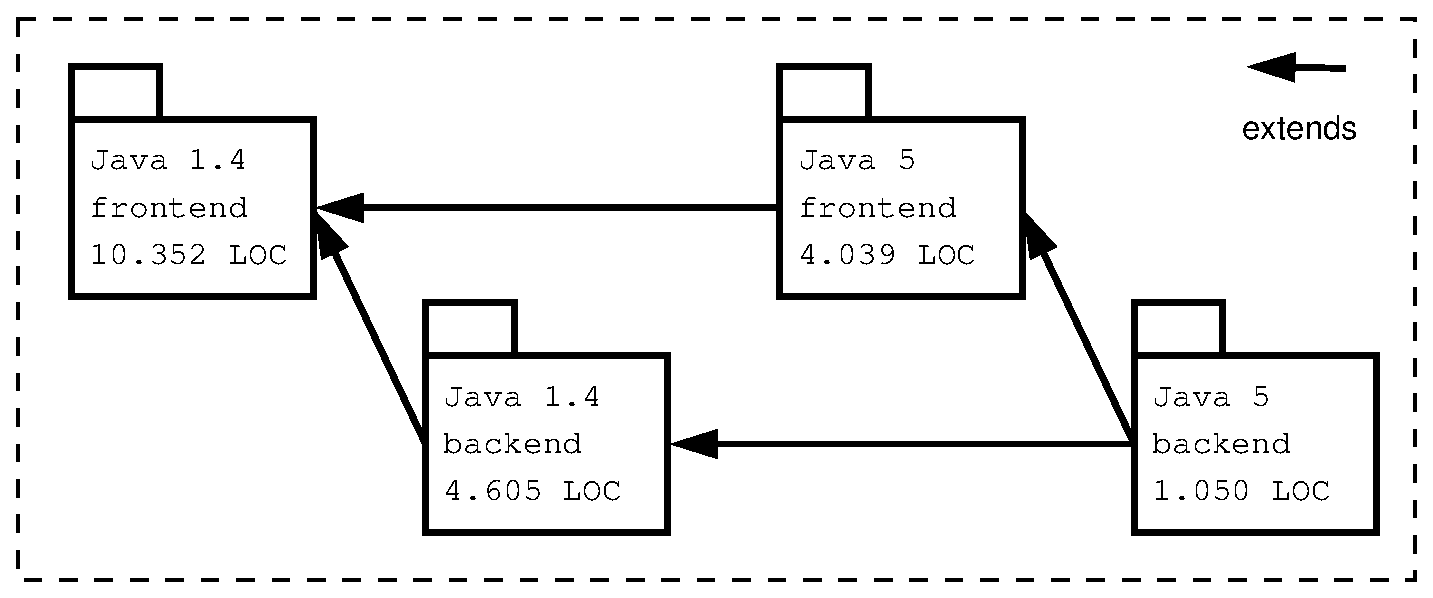
\includegraphics{figures/MainComponents}
    }
    \caption{The main components of JastAddJ}
    \label{MainComponents}
  \end{center}
\end{figure}

The components themselves are composed of AST "`base"' classes, and the
aspects that introduce the ITDs to the said classes. The AST classes
directly or indirectly extend the classes \texttt{ASTNode}, \texttt{List}, and \texttt{Opt},
which form the JastAdd framework classes. 

Since there is no module system each component is represented as a
directory of reusable source files that are combined using build files. The
Java 5 frontend is an extension to the Java 1.4 frontend, reusing its
source file, while specifying Java 5 language features as an increment to
the Java 1.4 frontend. A build file to create a Java 1.4 semantic checker
will thus only include files from the Java 1.4 folder, while a build file
for a Java 5 semantic checker includes files from both folders. The
backends are extensions to the frontends and reuse source files in a
similar manner.  By changing which files to include in the build it is
possible to build four different tools from these components.

Each frontend can be further divided into the following subcomponents: a
parser that builds an AST, a bytecode reader that reads class files, and a
semantic analyzer or code generator. The parser is generated from a context
free grammar, the bytecode reader is written in plain Java, and the
analyzers and code generators are implemented using attribute grammars and
inter-type declarations.

The architecture has a few problems that can be elegantly solved using a
module system. First, the different variants of the compiler can not
coexist in the same system since ITDs destructively update the class
hierarchy. This is handled with an ugly hack where multiple build files and
scripts are used generate compilers to different packages.  Second, the
bytecode readers are implemented in plain Java in a fashion which
unfortunately makes them quite hard to extend and we therefore use
different implementations of the reader in the Java 1.4 frontend and the
Java 5 frontend. This is handled by including different versions of source
files in the build for the Java 5 frontend and excluding some of the files
in the Java 1.4 frontend. Third, the systems are composed into one global
namespace which is terrible from an information hiding point of view.

\subsection{Applying Modules}

To remedy the problems detailed above, we apply the module system to
the JastAddJ compiler. We have refactored the components such that:

\begin{enumerate}
\item {The JastAdd framework classes reside in their own module.}
\item {The AST classes in the frontend components have been separated from the aspects, and extend the JastAdd framework module.}
\item {The Java 1.5 frontend extends the 1.4 frontend, and similarly with the backends and the AST modules}
\item {Dependencies between the modules were explicitly defined by the use of imports in the module declarations.}
	
\end{enumerate}

\begin{figure}[htb!]
  \begin{center}
    \resizebox{3in}{!}{
      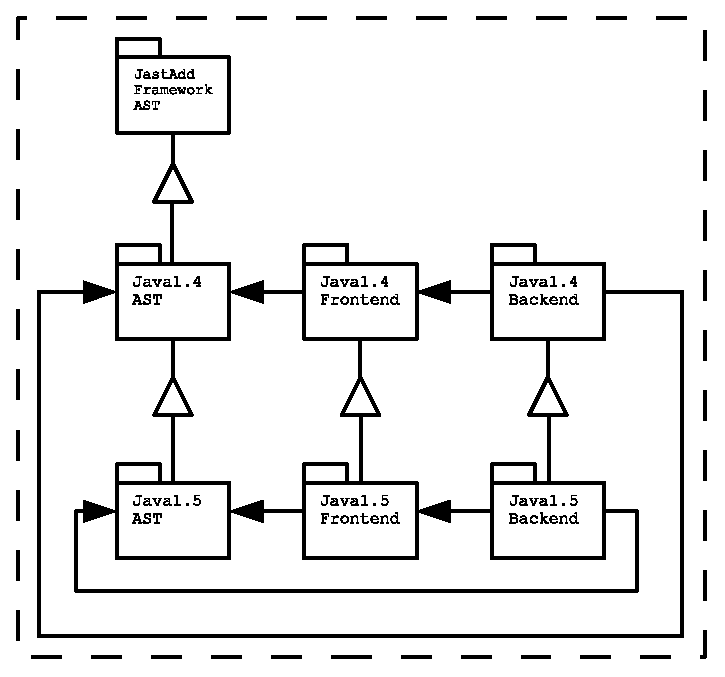
\includegraphics{figures/ModuleMainComponents}
    }
    \caption{JastAddJ refactored to use modules}
    \label{ModuleMainComponents}
  \end{center}
\end{figure}

Other than the necessary changes to use modules, it was also necessary to change the 
access modifiers of several ITDs from package private to public, to allow the 
access of these ITDs from outside their module. 

An example compiler application that uses the JastAddJ with modules is shown in the example below.
The module for the compiler application imports a frontend and a backend, and since the backend 
also imports an instance of the frontend, the \texttt{javacompiler} module contains a merge
operation that allows the java compiler and the backend to share the frontend classes.

\begin{lstlisting}[caption={JastAddJ Compiler Application}]
//file javacompiler.module
module javacompiler;
import own java15frontend as frontend;
import own java15backend as backend;
//merge the frontends to point to the same instance
merge frontend, backend::frontend as java15frontend frontend;
\end{lstlisting}

\subsection{Evaluation}

%Shows dependencies explicitly, information hiding, enables sharing through merge
The addition of modules to JastAddJ has made the dependencies of the components
explicit, and will lessen the chance of inadrvetently introducing dependencies 
in the future. 

%everything used to be globally visible
%  modules improves information hiding 
%    (concrete example would be nice)
%    percent that became non-global
Information hiding among the components of the system has also benefited from
the introduction of modules. In the previous system, the class files produced from
compilation all belong to the same package, which means that a package private access modifier
is equivalent to a public modifier. Though several ITDs needed to be changed from 
package private to public to allow access from outside, a great majority remained private to
the module. As an example, in the Java 1.4 frontend, 24 ITDs (including synthesized attributes)
were changed from package private to public to allow other modules to access them. This is a small number 
compared to the total number of synthesized attributes alone (541) that were package private in the pre-module version.
This has effectively reduced the public ITD signature of the the Java 1.4 frontend to 5\% of its previous state.

%enables variants with different sets of ITDs
%  examples


%enables variants with replaced/overridden classes
%  example: bytecode reader
%  (reason, monolithic implementation not suitable for extension, therefore
%  replacement easier)
The use of aspect overriding has allowed the Java 1.5 bytecode parser aspects in the Java 1.5 frontend to
override the corresponding aspects in the Java 1.4 frontend without the build file hacks that involved
excluding the Java 1.4 bytecode parser files when building the 1.5 compiler. This demonstrates that
aspect overriding solves a problem that arises in a real aspect oriented system, as opposed to 
hypothetical examples.s


%can we characterize the typical changes needed?
%how intrusive/global were the changes?
The changes required to introduce modules into JastAddJ were minimal: just the addition of the module 
declarations in \texttt{.module} files, the module membership specifications in the existing compilation units,
and a change to the access modifiers of some ITDs to allow inter-access. Given the benefits of instantiation, 
module composition and information hiding, this is a relatively small price to pay.

%eliminate cycles as a side-effect
%  required by the module system
%  architecture improved/ should have been done that way from the beginning
%  in retrospect
The use of \textbf{own} module instances will also benefit the architecture of JastAddJ,
since cyclic dependencies that involve \textbf{own} instances will cause an error to
be raised by the compiler. This provides a compile-time architecture check to avoid cyclic dependencies,
and would allow the early detection of decisions that would have caused unnecessarily
tight coupling between the components.

%many properties
%are global even though a more local scope would improve information hiding.

%improve extensibility and information hiding



 
 


\section{Related Work}
\label{section:related}
This is the related lit section.

iJAM for module instantiation \cite{iJAM}.

Modules as OO Types \cite{modulesastypes}.

JastAdd \cite{jastadd}

Open Modules for AJ \cite{openmodulesaj}

CaesarJ for aspect deployment \cite{caesarj}

Aspectual collaborations \cite{lieberherr03aspectual}

Aspectual mixin layers (for aspect refinement) \cite{aspectualmixinlayers}.
Ditto for virtual classes \cite{virtualclasses89}

Hyper/J for merge \cite{hyperj}

AOP and modularity \cite{aopmodularreasoning}

FOP \cite{fopstepwiserefinement}

XPIs (in case interfaces come up) \cite{xpi}

AspectJ \cite{overviewaspectj}

Composition filters \cite{compositionfilters}

\section{Conclusions}
\label{section:conclusions}
We have presented a module system that improves extensibility and
information hiding when using ITDs. Instantiation enables multiple
variants of a base system, each with its own set of applied ITDs. Imports
and exports enable better support for access control improving information
hiding. An important consequence of these features is that they remove some
deficiencies of using plain ITDs compared to a visitor based solution.

The module system has been implemented as an extension to the JastAdd
system, an aspect-oriented attribute grammar extension to Java, which
supports ITDs as one of its major modularization mechanisms. The solution
is purely compile-time and generates class files that can be executed on
a traditional JVM without explicit support for modules.

To evaluate the module system on a realistic system we retrofitted the
JastAdd Extensible Java Compiler (JastAddJ) to use modules. It is a medium
sized application of more than 21.000 lines of code which is designed using
the somewhat extreme viewpoint that the class hierarchy does not contain
any behavior but modularly added using ITDs. Minor changes to the
implementation enabled us to create a family of compilers that can coexist
in the same system using modules compared to the previous solution using an
ugly build file hack. Moreover, it enabled us to limit the scope of many
properties that were global in the original implementation.

As future work we will experiment with using the module instantiation
features to further enhance the reuse of ITDs. One can for instance
envision a situation where ITDs are multiply instantiated in different
modules of the same compiler rather than only across tool boundaries.


%ACKNOWLEDGMENTS are optional
\section{Acknowledgements}
\label{section:acknowledgements}
These are the acknowledgements.
%
% The following two commands are all you need in the
% initial runs of your .tex file to
% produce the bibliography for the citations in your paper.
\bibliographystyle{abbrv}
\bibliography{sigproc}  % sigproc.bib is the name of the Bibliography in this case
% You must have a proper ".bib" file
%  and remember to run:
% latex bibtex latex latex
% to resolve all references
%
% ACM needs 'a single self-contained file'!
%
\end{document}